\documentclass[aspectratio=169]{beamer}
\usepackage{tikz}
\usepackage{graphicx}
\usepackage[spanish]{babel}
\usepackage{geometry}
\usepackage[absolute,overlay]{textpos}

\usetikzlibrary{shapes.geometric}
\usetikzlibrary{shapes.arrows}
\usetikzlibrary{overlay-beamer-styles}
\setbeamertemplate{navigation symbols}{}

\setbeameroption{show notes on second screen=right}

\definecolor{blue1}{RGB}{126,126,206}
\definecolor{blue2}{RGB}{87,87,192}
\definecolor{blue3}{RGB}{51,51,178}
\definecolor{blue4}{RGB}{27,26,107}

\usepackage{color}
\definecolor{dkgreen}{rgb}{0,0.6,0}
\definecolor{gray}{rgb}{0.5,0.5,0.5}
\definecolor{mauve}{rgb}{0.58,0,0.82}
\definecolor{background}{rgb}{0.95, 0.95, 0.95}
\definecolor{numb}{rgb}{0.5,0.5,0.5} % grey color for numbers
\definecolor{punct}{rgb}{0,0,0}       % black color for punctuation
\definecolor{delim}{rgb}{0.08,0.52,0.8} % blue color for delimiters


\usepackage[
    backend=biber,
    sorting=ynt]{biblatex}
\addbibresource{biblio.bib}

\usepackage{listings}
\lstdefinelanguage{text}{
    basicstyle=\normalfont\ttfamily,
    moredelim=[is][\textcolor{blue}]{\#}{\#}, % Delimiter for bold text
}
\lstdefinelanguage{json}{
    moredelim=[is][\textcolor{blue}]{\#}{\#}, % Delimiter for bold text
    basicstyle=\small\ttfamily,
    numbers=left,
    numberstyle=\scriptsize,
    stepnumber=1,
    numbersep=8pt,
    showstringspaces=false,
    breaklines=true,
    frame=lines,
    backgroundcolor=\color{background},
    literate=
     *{0}{{{\color{numb}0}}}{1}
      {1}{{{\color{numb}1}}}{1}
      {2}{{{\color{numb}2}}}{1}
      {3}{{{\color{numb}3}}}{1}
      {4}{{{\color{numb}4}}}{1}
      {5}{{{\color{numb}5}}}{1}
      {6}{{{\color{numb}6}}}{1}
      {7}{{{\color{numb}7}}}{1}
      {8}{{{\color{numb}8}}}{1}
      {9}{{{\color{numb}9}}}{1}
      {:}{{{\color{punct}{:}}}}{1}
      {,}{{{\color{punct}{,}}}}{1}
      {\{}{{{\color{delim}{\{}}}}{1}
      {\}}{{{\color{delim}{\}}}}}{1}
      {[}{{{\color{delim}{[}}}}{1}
      {]}{{{\color{delim}{]}}}}{1},
  keywordstyle=\color{blue},
  commentstyle=\color{dkgreen},
  stringstyle=\color{mauve},
}

\lstset{
    language=text,
    showstringspaces=false,
    breaklines=true
}
% \lstset{frame=tb,
%   language=json,
%   aboveskip=3mm,
%   belowskip=3mm,
%   showstringspaces=false,
%   columns=flexible,
%   basicstyle={\small\ttfamily},
%   numbers=none,
%   numberstyle=\tiny\color{gray},
%   breaklines=true,
%   breakatwhitespace=true,
%   tabsize=3
% }

\usepackage{svg}

% \usetheme{Warsaw}
\usecolortheme{whale}
\title{Bases de Datos}
\subtitle{Introducci\'on a las Bases de Datos Relacionales y No Relacionales}

\author[Garc\'ia L., Cardentey V. M.]{ Lic. Andy Ledesma Garc\'ia \\ 
Lic. V\'ictor M. Cardentey Fundora \\ 
Dra. Lucina Garc\'ia Hern\'andez}

\institute[MATCOM-UH]{
    Departamento de Computaci\'on\\
    Facultad de Matem\'atica y Computaci\'on\\
    Universidad de La Habana\\[3mm]
    Licenciatura en Ciencia de Datos
}

\date[]{23 de enero de 2024}

\begin{document}
\maketitle
\begin{frame}{¿Qu\'e tan grande es YouTube?}

    \begin{columns}[T]
        \begin{column}{0.48\textwidth}
            \begin{overlayarea}{\linewidth}{\textheight}
                \vspace{17mm}

                \begin{itemize}
                    \item<1-> 500 horas de video subidas cada minuto
                    \item<2-> 720000 horas de video subidas cada d\'ia
                    \item<3-> Se necesitan \textcolor{red}{82 a\~nos} para ver el contenido de un solo d\'ia
                \end{itemize}
            \end{overlayarea}

        \end{column}

        \begin{column}{0.48\textwidth}
            \vspace{17mm}
            
            \includegraphics<3->[width=\textwidth]{img/skelly.jpg}
        \end{column}
    \end{columns}
\end{frame}

{
\setbeamertemplate{background} 
{
    
\includegraphics[width=\paperwidth,height=\paperheight]{img/Big-tech-banking-LatAm.jpg}
}
\begin{frame}
\end{frame}
}

\begin{frame}{Motivaci\'on}
    \begin{block}{Problemas a resolver}
        \begin{itemize}
            \item<2-> Garantizar la persistencia de los datos generados por aplicaciones y dispositivos.
            \item<3-> Utilizar grandes cantidades de datos de forma eficiente.
        \end{itemize}
    \end{block}
    
    \vspace{10pt}

    \centering
    \begin{tikzpicture}
        \onslide<2->{
        \node at (1.4,6.4) {\tiny \bf {Apps Web}} ;
        \node[inner sep=0pt] (web) at (1.4,5.6) {
            
\includegraphics[width=1.3cm]{img/web.png}
        };

        \node at (-0.1, 5.5) {\tiny \bf {Apps Escritorio}};
        \node[inner sep=0pt] (desktop) at (0,4.7){
            
\includegraphics[width=1.3cm]{img/desktop.png}
        };

        \node at (0,2.6) {\tiny \bf {Apps m\'oviles}};
        \node[inner sep=0pt] (mobile) at (0,3.4){
            
\includegraphics[width=1.3cm]{img/mobile.png}
        };

        \node at (1.4,1.7) {\tiny \bf {Internet de las cosas}};
        \node[inner sep=0pt] (iot) at (1.4,2.5) {
            
\includegraphics[width=1.3cm]{img/iot.png}
        };

        \node at (4,5) {\tiny \bf {Datos}};
        \node[inner sep=0pt] (database) at (4,4) {
            
\includegraphics[width=1.8cm]{img/data.png}
        };

        }

        \onslide<2>{
            \draw[->,thick] (web.south east) -- (3.1,4.3);
            \draw[->,thick] (desktop.east) -- (3.1,4.1);
            \draw[->,thick] (mobile.east) -- (3.1,3.8);
            \draw[->,thick] (iot.north east) -- (3.1,3.6);
        }

        \onslide<3->{
            \draw[<->,thick] (web.south east) -- (3.1,4.3);
        \draw[<->,thick] (desktop.east) -- (3.1,4.1);
        \draw[<->,thick] (mobile.east) -- (3.1,3.8);
        \draw[<->,thick] (iot.north east) -- (3.1,3.6);

        \node at (6.5,6.4) {\tiny \bf {Reportes}};
        \node[inner sep=0pt] (report) at (6.5, 5.6) {
            
\includegraphics[width=1.3cm]{img/report.png}
        };
        \node at (7.9,4.9) {\tiny \bf {Modelos de IA}};
        \node[inner sep=0pt] (ai) at (7.9, 4.1) {
            
\includegraphics[width=1.3cm]{img/ia.png}
        };
        \node at (6.5,1.7) {\tiny \bf {Recomendaciones}};
        \node[inner sep=0pt] (ranking) at (6.5, 2.5) {
            
\includegraphics[width=1.3cm]{img/ranking.png}
        };
        
        \draw[->,thick] (4.9,4.3) -- (report.south west);
        \draw[->,thick] (database.east) -- (ai.west);
        \draw[->,thick] (4.9,3.6) -- (ranking.north west);
        }
        
        
    \end{tikzpicture}
  
  
\end{frame}

\begin{frame}{¿C\'omo?}
    \begin{block}<2>{}
        La forma m\'as sencilla de almacenar datos es escribirlos en un fichero
    \end{block}
    \vspace{5mm}

    \centering
    \includegraphics<2>[width=50mm, height=50mm]{img/csv.png}

    \note<2>{@NOTE seguramente han trabajado con ficheros previamente}

    \note<2>{@NOTE noten c\'omo se encuentran los datos almacenados (formato csv). Han trabajado con csv antes?}
\end{frame}


\begin{frame}{Sistemas orientados a ficheros}
   
    \begin{columns}[T]
        \begin{column}{0.30\linewidth}
            \begin{block}
                
                \begin{tabular}{c c c}
    
                    
\includegraphics[width=1cm]{img/list.png}
                    
                    & 
\includegraphics[width=1cm]{img/list.png}
                    & 
\includegraphics[width=1cm]{img/list.png}\\
    
                    
\includegraphics[width=1cm]{img/list.png}
                    & 
\includegraphics[width=1cm]{img/list.png}
                    & 
\includegraphics[width=1cm]{img/list.png}\\
    
                    
\includegraphics[width=1cm]{img/list.png}
                    & 
\includegraphics[width=1cm]{img/list.png}
                    & 
\includegraphics[width=1cm]{img/list.png}\\
    
    
                    ... & ... & ...\\
    
                    
\includegraphics[width=1cm]{img/list.png}
                    & 
\includegraphics[width=1cm]{img/list.png}
                    & 
\includegraphics[width=1cm]{img/list.png}\\
    
                    
\includegraphics[width=1cm]{img/list.png}
                    & 
\includegraphics[width=1cm]{img/list.png}
                    & 
\includegraphics[width=1cm]{img/list.png}\\
    
                \end{tabular}
            \end{block}
            
    \end{column}

    


        \begin{column}{0.68\linewidth}
            \begin{block}{Caracter\'isticas}
                \begin{itemize}
                    \item Se crean nuevos ficheros a medida que se crean nuevos tipos de registros o se eliminan los ficheros.
                    \item Cada fichero se opera de forma independiente del resto de archivos en almacenamiento.
                \end{itemize}
                 
            \end{block}
            \begin{alertblock}<2->{Limitaciones}
                \begin{itemize}
                    \item<2-> Baja eficiencia
                    \item<3-> Gran redundancia de los datos
                    \item<4-> Pobre control sobre los datos
                    \item<5-> Capacidades inadecuadas de manipulaci\'on de datos
                \end{itemize}
            \end{alertblock}
        \end{column}

    \end{columns}

    \note<1>{@NOTE fue el 1er recurso digital para almacenar grandes vol\'umenes de datos}

    \note<1>{@NOTE por ``eliminar'' no solamente me refiero a borrar, sino tambi\'en a ignorar}

    \note<1>{@NOTE no hay manera de enlazar esos ficheros}

    \note<2>{@NOTE b\'usqueda secuencial}

    \note<3>{@NOTE debido a q no est\'an relacionados. Por qu\'e creen q esto sea una limitaci\'on? Esto lleva f\'acilmente a inconsistencias}

    \note<4>{@NOTE producto de la redundancia y la no relaci\'on entre los datos}

    \note<5>{@NOTE cada desarrollador deb\'ia implementar sus propias operaciones de manipulaci\'on de datos}
\end{frame}
\begin{frame}{Bases de datos}
    \begin{overlayarea}{\linewidth}{\textheight}
        \begin{onlyenv}
            \begin{block}{}
                \begin{quote}
                    ``... una base de datos es una colecci\'on auto-descriptiva de registros integrados."
                    \hspace{1em plus 1fill}---Allen Taylor
                \end{quote}
            \end{block}
      \end{onlyenv}
    \end{overlayarea}
   

    
\end{frame}

\begin{frame}{Bases de datos}

    \begin{overlayarea}{\linewidth}{\textheight}
        \begin{onlyenv}
            \begin{block}{}
                \begin{quote}
                    ``... una base de datos es una colecci\'on auto-descriptiva de \textcolor{red}{registros} integrados."
                    \hspace{1em plus 1fill}---Allen Taylor
                \end{quote}
                
                \textcolor{red}{Registro}: datos espec\'ificos sobre una entidad u objeto de inter\'es
            \end{block}
      \end{onlyenv}
      \vspace{8mm}
      \centering
      \begin{tabular}{|c|c|c|c|c|}
          \hline
          98082200205 & Jos\'e & P\'erez & 22/08/98\\
          \hline
      \end{tabular}
    \end{overlayarea}
   


    
\end{frame}

\begin{frame}{Bases de datos}

    \begin{overlayarea}{\linewidth}{\textheight}
        \begin{onlyenv}
            \begin{block}{}
            \begin{quote}
                ``... una base de datos es una colecci\'on \textcolor{red}{auto-descriptiva} de registros integrados."
                \hspace{1em plus 1fill}---Allen Taylor
            \end{quote}
    
            \textcolor{red}{Auto-descriptiva}: se almacenan metadatos (la descripci\'on de su estructura) dentro
            del diccionario de datos de la propia base de datos.
        \end{block}
      \end{onlyenv}
      
          \vspace{5mm}
          \large \textbf{Persona}
          \vspace{2mm}
          \centering{
          
      
          \begin{tabular}{|c|c|c|c|}
              \hline
              CI : \textcolor{blue}{\texttt{string}} & Nombre : \textcolor{blue}{\texttt{string}} & Apellido : \textcolor{blue}{\texttt{string}} & F. Nacimiento : \textcolor{blue}{\texttt{date}} \\ 
              \hline
              98082200205 & Jos\'e & P\'erez & 22/08/98 \\
              \hline
          \end{tabular}
          }
    \end{overlayarea}
    


    % \large \textbf{Cuenta}
    % \vspace{2mm}
    % \centering{
    

    % \begin{tabular}{|c|c|}
    %     \hline
    %     No. Cuenta : \textcolor{blue}{\texttt{string}} & Balance : \textcolor{blue}{\texttt{decimal}}\\
    %     \hline
    %     8976 & 270.98\\
    %     \hline
    % \end{tabular}
    % }
   

    
\end{frame}



\begin{frame}{Bases de datos}
    \begin{overlayarea}{\linewidth}{\textheight}
        \begin{onlyenv}
            \begin{block}{}
                \begin{quote}
                    ``... una base de datos es una colecci\'on auto-descriptiva de registros \textcolor{red}{integrados}."
                    \hspace{1em plus 1fill}---Allen Taylor
                \end{quote}
                \textcolor{red}{Integrados}: no solo contiene los datos sino tambi\'en las interrelaciones
                 que se establecen entre estos.
            \end{block}
      \end{onlyenv}

      \vspace{5mm}
    \large \textbf{Persona}
    \vspace{2mm}
    \centering{
    

    \begin{tabular}{|c|c|c|c|}
        \hline
        CI : \textcolor{blue}{\texttt{string}} & Nombre : \textcolor{blue}{\texttt{string}} & Apellido : \textcolor{blue}{\texttt{string}} & F. Nacimiento : \textcolor{blue}{\texttt{date}} \\ 
        \hline
        \textcolor{red}{98082200205} & Jos\'e & P\'erez & 22/08/98 \\
        \hline
    \end{tabular}
    }

    \vspace{5mm}


    \large \textbf{Cuenta}

    \vspace{2mm}
    \centering{
    \begin{tabular}{|c|c|c|}
        \hline
        No. Cuenta : \textcolor{blue}{\texttt{string}} & Balance : \textcolor{blue}{\texttt{decimal}} & CI Due\~no : \textcolor{blue}{\texttt{string}} \\
        \hline
        8976 & 270.98 & \textcolor{red}{98082200205} \\
        \hline
    \end{tabular}
    }
    \end{overlayarea}
    

    
\end{frame}





\begin{frame}{Un cambio de enfoque}
    \begin{overlayarea}{\linewidth}{\textheight}
        \begin{onlyenv}
            \begin{block}{}
                
                En los sistemas orientados a ficheros los humanos tienen el control sobre los ficheros  
            \end{block}
        \end{onlyenv}

        \vspace{10mm}

        \centering
        \includegraphics<2>[height=50mm, width=80mm]{img/filesystem.png}
    \end{overlayarea}
\end{frame}


\begin{frame}{Un cambio de enfoque}
    \centering
    \begin{tikzpicture}
        \node at (0,3.7) {\tiny \bf {Usuario}} ;
        \node[inner sep=0pt] (user) at (0,3) {
            
\includegraphics[width=1.3cm]{img/user.png}
        };


        \node at (6,3.7) {\tiny \bf {Fichero}} ;
        \node[inner sep=0pt] (file) at (6,3) {
            
\includegraphics[width=1.3cm]{img/file.png}
        };

        \draw[<->,thick] (user.east) -- (file.west);
    \end{tikzpicture}

    El usuario interact\'ua directamente con los ficheros

    \vspace{20pt}
    \centering
    \begin{tikzpicture}
        \node at (0,3.7) {\tiny \bf {Usuario}} ;
        \node[inner sep=0pt] (user) at (0,3) {
            
\includegraphics[width=1.3cm]{img/user.png}
        };

        \node at (3,3.7) {\tiny \bf {Software}} ;
        \node[inner sep=0pt] (dbms) at (3,3) {
            
\includegraphics[width=1.3cm]{img/dbms.png}
        };

        \node at (6,3.7) {\tiny \bf {Base de datos}} ;
        \node[inner sep=0pt] (database) at (6,3) {
            
\includegraphics[width=1.3cm]{img/database.png}
        };

        \draw[<->,thick] (user.east) -- (dbms.west);
        \draw[<->,thick] (dbms.east) -- (database.west);
    \end{tikzpicture}
    
    El usuario interact\'ua con la base de datos mediante
    \textit{software}
   
\end{frame}
\begin{frame}{¿Qu\'e es este \textit{software}?}



    \begin{block}{Sistemas de gesti\'on de bases de datos (SGBD)}
        \begin{quote}
            ``Un \textcolor{red}{sistema de gesti\'on de bases de datos}
            es un sistema computacional que proporciona
            \textcolor{red}{funcionalidades, medios o servicios para manipular} y, en particular,
            \textcolor{red}{manejar todos los accesos} a una base de datos o una colecci\'on
            de bases de datos." \hspace{1em plus 1fill}---C. J. Date
        \end{quote}
    \end{block}
\end{frame}


\begin{frame}{Superando limitaciones}
       
            \begin{block}{}
                \begin{itemize}
                    \item<1-> \textbf{Persistentes}: los datos permanecen en memoria externa
                    \item<2-> \textbf{Masivos}: manejan terabytes/petabytes de datos
                    \item<3-> \textbf{Eficientes}: operaciones eficientes gracias al uso de estructuras de datos y algoritmos
                    \item<4-> \textbf{Multi-usuarios}: protocolos para la gesti\'on de accesos concurrentes
                    \item<5-> \textbf{Seguros}: consistentes ante accesos por usuarios no autorizados y fallos del sistema
                    \item<6-> \textbf{Disponibles}: al 99.99999\%
                \end{itemize}
            \end{block}
               
\end{frame}


\begin{frame}{Superando expectativas}
    \begin{block}{Conveniencia de los SGBD}
        \begin{itemize}
            \item<2-> \textbf{Independencia f\'isica de datos}: admiten el cambio de la forma de
            almacenamiento de los datos, pero la estructura de la base de datos y las operaciones
            definidas sobre ella no cambian.
            \item<3-> \textbf{Independencia l\'ogica de datos}: proporcionan lenguajes de consulta declarativos, se define
            lo que se desea pero no c\'omo alcanzarlo.
        \end{itemize}
        
    \end{block}

\end{frame}


\begin{frame}{Superando las expectativas}
    \centering
    \begin{tikzpicture}
        \node at (1.4,7) {\tiny \bf {Usuario de SGBD}} ;
        \node[inner sep=0pt] at (1.4,5.8) {
            
\includegraphics[width=1.8cm]{img/hface.png}
        };

        \node at (1.4,4.3) {\tiny \bf {Desarrollador de SGBD}} ;
        \node[inner sep=0pt] at (1.4,3.2) {
            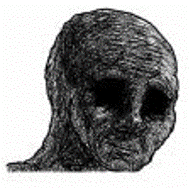
\includegraphics[width=1.8cm]{img/sface.png}
        };

        \draw[-,thick] (0.3, 4.6) -- (7,4.5);
        \draw[-,thick] (2.7, 2) -- (2.7,7.4);

        \node at (5,5.8) {Lenguaje declarativo};
        \node at (5,4.3) {Estructuras de datos};%\\Algoritmos\\Optimizaci\'on\\Compilaci\'on\\Gesti\'on de ficheros};
        \node at (5,3.8) {Algoritmos};%\\Algoritmos\\Optimizaci\'on\\Compilaci\'on\\Gesti\'on de ficheros};
        \node at (5,3.3) {Optimizaci\'on};%\\Algoritmos\\Optimizaci\'on\\Compilaci\'on\\Gesti\'on de ficheros};
        \node at (5,2.8) {Compilaci\'on};%\\Algoritmos\\Optimizaci\'on\\Compilaci\'on\\Gesti\'on de ficheros};
        \node at (5,2.3) {Gesti\'on de ficheros};%\\Algoritmos\\Optimizaci\'on\\Compilaci\'on\\Gesti\'on de ficheros};

    \end{tikzpicture}
\end{frame}
\begin{frame}{Sistemas de bases de datos (SBD)}
  
    \centering
    \begin{tikzpicture}<1->
        \node at (0,3.7) {\tiny \bf {Usuario}} ;
        \node[inner sep=0pt] (user) at (0,3) {
            
\includegraphics[width=1.3cm]{img/user.png}
        };

        \node at (3,3.7) {\tiny \bf {Aplicaci\'on}} ;
        \node[inner sep=0pt] (desktop) at (3,3) {
            
\includegraphics[width=1.3cm]{img/desktop.png}
        };

        \node at (6,3.7) {\tiny \bf {SGBD}} ;
        \node[inner sep=0pt] (dbms) at (6,3) {
            
\includegraphics[width=1.3cm]{img/dbms.png}
        };

        \node at (9,3.7) {\tiny \bf {Base de datos}} ;
        \node[inner sep=0pt] (database) at (9,3) {
            
\includegraphics[width=1.3cm]{img/database.png}
        };

        \draw[<->,thick] (user.east) -- (desktop.west);
        \draw[<->,thick] (desktop.east) -- (dbms.west);
        \draw[<->,thick] (dbms.east) -- (database.west);
    \end{tikzpicture}
    \vspace{10pt}
    \begin{block}<2->{}
        \begin{quote}
            ``Un \textcolor{red}{sistema de base de datos} es un 
            \textcolor{red}{sistema computacional de mantenimiento de registros}, 
            que se dise\~na para manejar grandes cantidades de informaci\'on."
            \hspace{1em plus 1fill}---C. J. Date
        \end{quote}
       
    \end{block}

    \begin{block}<3->{Funciones}
        \begin{columns}[T]
            \begin{column}{0.48\linewidth}
                \begin{itemize}
                    \item Insertar datos
                    \item Editar datos
                \end{itemize}
            \end{column}
            \begin{column}{0.48\linewidth}
                \begin{itemize}
                    \item Eliminar datos
                    \item Consultar datos
                \end{itemize}
            \end{column}
            
        \end{columns}
    \end{block}
  
\end{frame}



\begin{frame}{Evoluci\'on de las tecnolog\'ias de la informaci\'on}

    \begin{overlayarea}{\linewidth}{\textheight}
        \vspace{10mm}
        \centering
    \begin{tikzpicture}[xscale=0.15]

        \node[rectangle, fill=blue, minimum width=14mm] at (0,0) {};
        \node[anchor=south, color=blue, inner sep=0pt] at (0.2,0.3) {\small 1980};

        \node[rectangle, fill=black!20, minimum width=14mm] at (10,0) {};
        \node[anchor=south, color=black!20, inner sep=0pt] at (10.2,0.3) {\small 1990};

        \node[rectangle, fill=black!20, minimum width=14mm] at (20,0) {};
        \node[anchor=south, color=black!20, inner sep=0pt] at (20.2,0.3) {\small 2000};

        \node[rectangle, fill=black!20, minimum width=14mm] at (30,0) {};
        \node[anchor=south, color=black!20, inner sep=0pt] at (30.2,0.3) {\small 2010};
    \end{tikzpicture}

    \vspace{20pt}

    \begin{columns}[T]
        \begin{column}{0.23\textwidth}
            \centering
            
\includegraphics[width=1.3cm]{img/sqldb_nb.png}\\
            Primeros sistemas gestores de bases de datos relacionales comerciales
        \end{column}
        \begin{column}{0.23\textwidth}
            \centering
            
\includegraphics[width=1.3cm]{img/sql.png}\\
            Est\'andar de lenguaje SQL
        \end{column}

        \begin{column}{0.23\textwidth}
            \centering
            
\includegraphics[width=1.3cm]{img/server.png}\\
            {Primeros servidores de bases de datos relacionales}
        \end{column}
        \begin{column}{0.23\textwidth}
            \centering
            
\includegraphics[width=1.3cm]{img/monitor.png}\\
            Procesamiento anal\'itico de datos
        \end{column}
    \end{columns}
    \end{overlayarea}
   

\end{frame}



\begin{frame}{Evoluci\'on de las tecnolog\'ias de la informaci\'on}
    \begin{overlayarea}{\textwidth}{\textheight}
        \vspace{10mm}
    \centering
    \begin{tikzpicture}[xscale=0.15]

        \node[rectangle, fill=black!20, minimum width=14mm] at (0,0) {};
        \node[anchor=south, color=black!20, inner sep=0pt] at (0.2,0.3) {\small 1980};

        \node[rectangle, fill=blue, minimum width=14mm] at (10,0) {};
        \node[anchor=south, color=blue, inner sep=0pt] at (10.2,0.3) {\small 1990};

        \node[rectangle, fill=black!20, minimum width=14mm] at (20,0) {};
        \node[anchor=south, color=black!20, inner sep=0pt] at (20.2,0.3) {\small 2000};

        \node[rectangle, fill=black!20, minimum width=14mm] at (30,0) {};
        \node[anchor=south, color=black!20, inner sep=0pt] at (30.2,0.3) {\small 2010};
    \end{tikzpicture}

    \vspace{20pt}

    \begin{columns}[T]
        \begin{column}{0.23\textwidth}
            \centering
            
\includegraphics[width=1.3cm]{img/website.png}\\
            Internet
        \end{column}
        \begin{column}{0.23\textwidth}
            \centering
            
\includegraphics[width=1.3cm]{img/online-store.png}\\
            Negocios online
        \end{column}

        \begin{column}{0.23\textwidth}
            \centering
            
\includegraphics[width=1.3cm]{img/xml.png}\\
            Modelo orientado a objetos\\ XML
        \end{column}
    \end{columns}
\end{overlayarea}

\end{frame}


\begin{frame}{Evoluci\'on de las tecnolog\'ias de la informaci\'on}
    \begin{overlayarea}{\textwidth}{\textheight}
        \vspace{10mm}
    \centering
    \begin{tikzpicture}[xscale=0.15]

        \node[rectangle, fill=black!20, minimum width=14mm] at (0,0) {};
        \node[anchor=south, color=black!20, inner sep=0pt] at (0.2,0.3) {\small 1980};

        \node[rectangle, fill=black!20, minimum width=14mm] at (10,0) {};
        \node[anchor=south, color=black!20, inner sep=0pt] at (10.2,0.3) {\small 1990};

        \node[rectangle, fill=blue, minimum width=14mm] at (20,0) {};
        \node[anchor=south, color=blue, inner sep=0pt] at (20.2,0.3) {\small 2000};

        \node[rectangle, fill=black!20, minimum width=14mm] at (30,0) {};
        \node[anchor=south, color=black!20, inner sep=0pt] at (30.2,0.3) {\small 2010};
    \end{tikzpicture}

    \vspace{20pt}

    \begin{columns}[T]
        \begin{column}{0.23\textwidth}
            \centering
            
\includegraphics[width=1.3cm]{img/warehouse.png}\\
            Data Warehousing
        \end{column}

        \begin{column}{0.23\textwidth}
            \centering
            
\includegraphics[width=1.3cm]{img/networking.png}\\
            Redes sociales
        \end{column}
        \begin{column}{0.23\textwidth}
            \centering
            
\includegraphics[width=1.3cm]{img/booking.png}\\
            Computaci\'on m\'ovil
        \end{column}

        \begin{column}{0.23\textwidth}
            \centering
            
\includegraphics[width=1.3cm]{img/big-data.png}\\
            Inicios del Big Data
        \end{column}

    \end{columns}
\end{overlayarea}

\end{frame}



\begin{frame}{Evoluci\'on de las tecnolog\'ias de la informaci\'on}
    \begin{overlayarea}{\textwidth}{\textheight}
        \vspace{10mm}
    \centering
    \begin{tikzpicture}[xscale=0.15]

        \node[rectangle, fill=black!20, minimum width=14mm] at (0,0) {};
        \node[anchor=south, color=black!20, inner sep=0pt] at (0.2,0.3) {\small 1980};

        \node[rectangle, fill=black!20, minimum width=14mm] at (10,0) {};
        \node[anchor=south, color=black!20, inner sep=0pt] at (10.2,0.3) {\small 1990};

        \node[rectangle, fill=black!20, minimum width=14mm] at (20,0) {};
        \node[anchor=south, color=black!20, inner sep=0pt] at (20.2,0.3) {\small 2000};

        \node[rectangle, fill=blue, minimum width=14mm] at (30,0) {};
        \node[anchor=south, color=blue, inner sep=0pt] at (30.2,0.3) {\small 2010};
    \end{tikzpicture}

    \vspace{20pt}

    \begin{columns}[T]
        
        \begin{column}{0.23\textwidth}
            \centering
            
\includegraphics[width=1.6cm]{img/noSQL.png}\\
            Sistemas gestores de bases de datos NoSQL
        \end{column}

        \begin{column}{0.23\textwidth}
            \centering
            
\includegraphics[width=1.3cm]{img/cloud-computing.png}\\
            Computaci\'on en la nube
        \end{column}
    \end{columns}
\end{overlayarea}

\end{frame}
\begin{frame}
\begin{textblock*}{\paperwidth}(0mm,0mm) % {block width} (coords)
    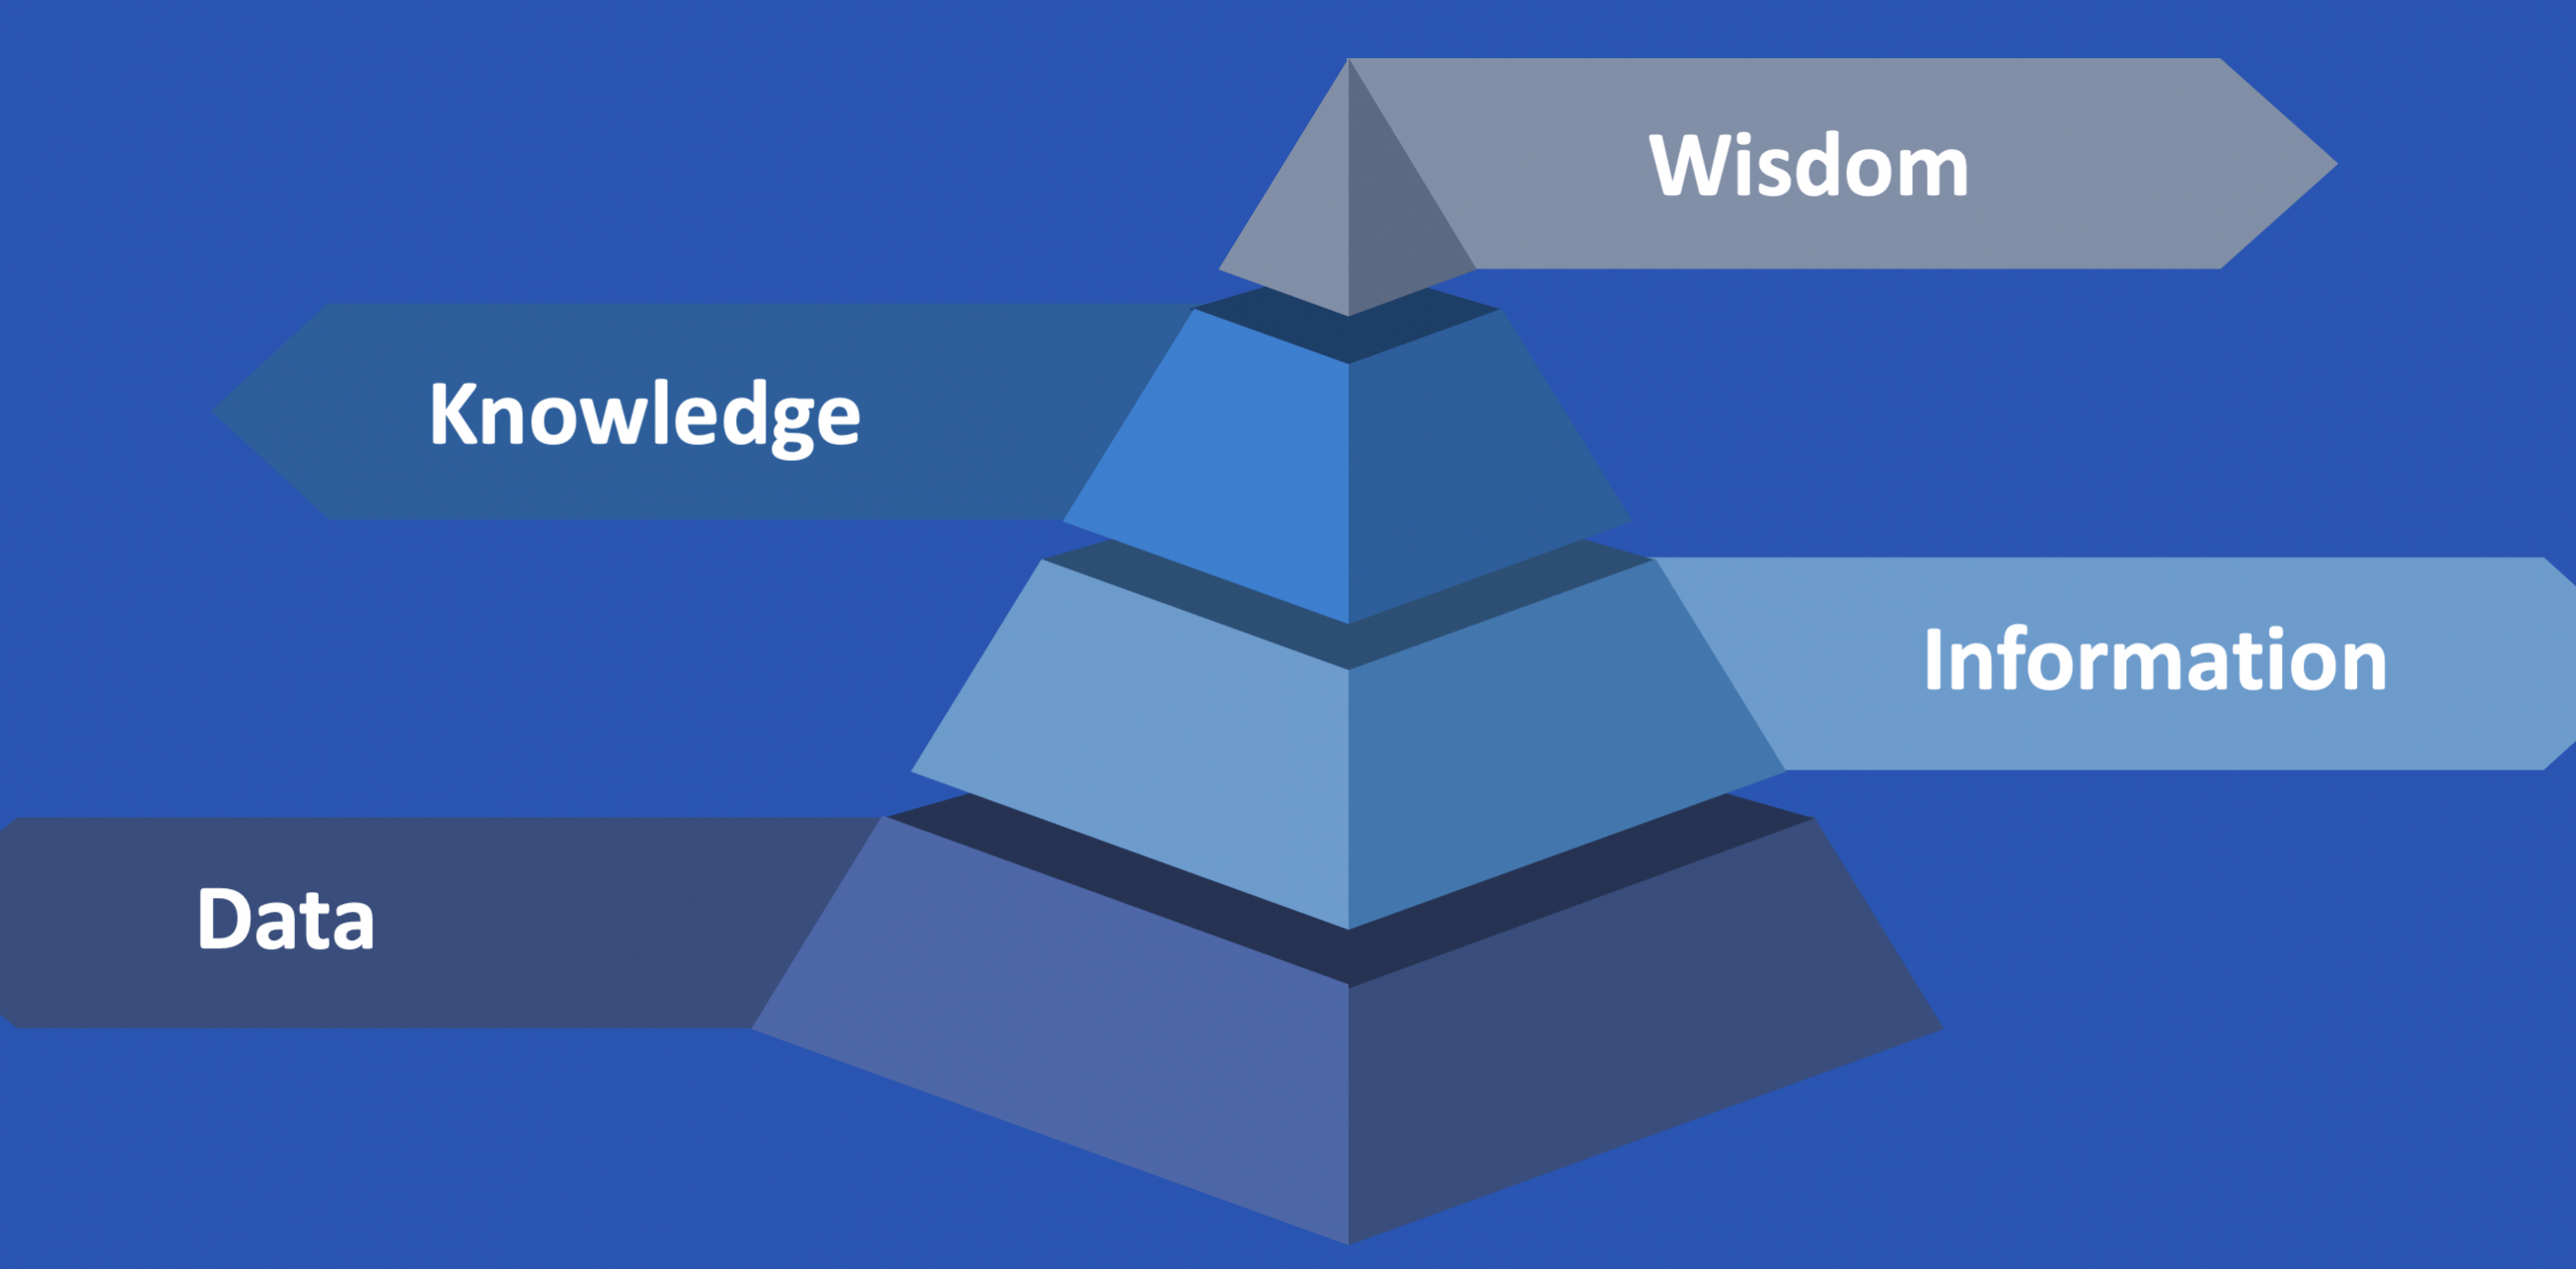
\includegraphics[width=\paperwidth,height=\paperheight]{img/hierarchy.png}
  \end{textblock*}
\end{frame}
\begin{frame}{Objetivos de la asignatura}
    % \begin{block}{Bases de datos relacionales}
    %     \begin{itemize}
    %         \item<1-> Orientadas a almacenar datos estructurados (datos tabulares)
    %         \item<2-> Basadas en el modelo relacional (modelo matem\'atico de datos)
    %         \item<3-> Permiten el procesamiento transaccional de datos
    %         \item<4-> Base de los sistemas de informaci\'on para la generaci\'on de conocimiento
    %     \end{itemize}
    % \end{block}

    \begin{block}{Proporcionar un conjunto de m\'etodos y herramientas para:}
        \pause
        \begin{itemize}[<+->]
            \item Dise\~nar e implementar bases de datos correctas
            \item Evaluar la calidad de bases de datos espec\'ificas
            \item Identificar la vigencia del modelo relacional y sus limitaciones
            \item Reconocer casos de uso para bases de datos no relacionales
        \end{itemize}        
    \end{block}

    \note<5>{@NOTE reformular en t\'erminos de insistir en la parte anal\'itica y en la diversidad de enfoques nosql}
\end{frame}
\begin{frame}{Estructura de la asignatura}
    % \begin{columns}[T]
    %     \begin{column}{0.24\linewidth}
    %         \begin{tikzpicture}
    %             \node[rectangle, fill=violet, minimum width=\linewidth] at (0,0) {};
    %         \end{tikzpicture}
    %         \centering
    %         An\'alisis de Requerimientos
    %     \end{column}
    %     \begin{column}{0.24\linewidth}
    %         \begin{tikzpicture}
    %             \node[rectangle, fill=cyan, minimum width=\linewidth] at (0,0) {};
    %         \end{tikzpicture}
    %         \centering
    %         Dise\~no Conceptual
    %     \end{column}
    %     \begin{column}{0.24\linewidth}
    %         \begin{tikzpicture}
    %             \node[rectangle, fill=green, minimum width=\linewidth] at (0,0) {};
    %         \end{tikzpicture}
    %         \centering
    %         Dise\~no\\ L\'ogico
    %     \end{column}
    %     \begin{column}{0.24\linewidth}
    %         \begin{tikzpicture}
    %             \node[rectangle, fill=blue, minimum width=\linewidth] at (0,0) {};
    %         \end{tikzpicture}
    %         \centering
    %         Dise\~no\\ F\'isico
    %     \end{column}
    \begin{overlayarea}{\linewidth}{\textheight}
        \vspace{5mm}
        \centering
        \begin{tikzpicture}
            \node<1->[rectangle, fill=blue1, minimum width=5cm, minimum height=8mm, text=white] at (0,0) {An\'alisis de Requerimientos};
            \node<2->[single arrow, fill=black, inner sep=6pt, rotate=270] at (0,-0.8){};
            \node<2->[rectangle, fill=blue2, minimum width=5cm, minimum height=8mm, text=white] at (0,-1.8) {Dise\~no Conceptual};
            \node<3->[single arrow, fill=black, inner sep=6pt, rotate=270] at (0,-2.6){};
            \node<3->[rectangle, fill=blue3, minimum width=5cm, minimum height=8mm, text=white] at (0,-3.6) {Dise\~no L\'ogico};
            \node<4->[single arrow, fill=black, inner sep=6pt, rotate=270] at (0,-4.4){};
            \node<4->[rectangle, fill=blue4, minimum width=5cm, minimum height=8mm, text=white] at (0,-5.4) {Dise\~no F\'isico};
        \end{tikzpicture}
            
    \end{overlayarea}
        
\end{frame}
\begin{frame}{Evaluaci\'on de la asignatura}
    \begin{columns}[T]
        \begin{column}{0.40\linewidth}
            \begin{block}{Evaluaci\'on Sistem\'atica}
        
                \begin{itemize}
                    \item Participaci\'on en clases
                    \item Entrega de tareas orientadas
                    \item Asistencia
                \end{itemize}
            \end{block}    
            \vspace{10pt}
            \begin{block}<2->{Nota Final}
                
                \begin{itemize}
                    \item Proyecto integrador
                    \item Opini\'on del profesor
                \end{itemize}
            \end{block}
        \end{column}
        
        \begin{column}{0.58\linewidth}
            
\includegraphics[width=0.8\textwidth, height=0.8\textheight]{img/eval.jpg}
        \end{column}
    \end{columns}

   
\end{frame}
\begin{frame}{Pr\'oximo encuentro}
            \begin{block}{Clase Pr\'actica}
                \begin{itemize}
                    \item Viernes, 2:55pm, aula 2
                    \item Instalar \textit{software}
                    \item Compartir bibliograf\'ia
                    \item \alert<2>{Orientaci\'on del proyecto}
                \end{itemize}
            \end{block}
            
            \centering
            \includegraphics[width=1cm]{img/telegram.png}
            
            \href{https://t.me/matcom_database_ds}{\textcolor{blue}{@matcom\_database\_ds}}
     
     \note<1>{@NOTE traigan laptops}
\end{frame}
\maketitle
\end{document}

% @TODO hacer q todos los ti'tulos sean Camel Case o no (elige uno)
% @TODO garantizar consistencia tambie'n en el punto despue's de cada item en un itemize